\chapter{Resultados e Discussões}
\label{cap:resultados}

Este capítulo apresenta os achados empíricos do estudo, com foco na experiência do usuário medida por \textit{Core Web Vitals} (coleta em campo, no cliente) e, de forma complementar, em diagnósticos laboratoriais do Lighthouse. Como contexto operacional, reporta-se também o consumo de CPU, memória e PIDs dos contêineres durante as execuções. A metodologia, o ambiente controlado e os procedimentos de coleta já foram descritos no Cap.~\ref{cap:estudo_caso_dev}; aqui concentramos a atenção em resultados e implicações.

\section{Resultados}
Os testes cobriram as duas variantes da WallTech (\acrshort{ssr}/\acrshort{mpa} em Next.js e \acrshort{csr}/\acrshort{spa} em React) nas páginas: inicial, resultados de busca e detalhes da notícia. Para cada cenário, foram realizados 10--15 carregamentos após \textit{warm-up}, e as leituras são analisadas por mediana (p50) e, quando pertinente, p95.

As fontes de dados utilizadas foram: {Web Vitals (núcleo), com \acrshort{ttfb}, \acrshort{fcp}, \acrshort{lcp}, \acrshort{cls}, \acrshort{inp} registrados no cliente e persistidos em NDJSON; e Lighthouse (apoio), com \acrshort{tbt} e principais oportunidades/auditorias de desempenho, além de verificações de Acessibilidade e SEO.

\subsection{Análise e Visualização dos Dados}
Os dados coletados, incluindo as métricas de \textit{Web Vitals} e as medições de recursos do servidor, foram exportados e analisados com o auxílio do Power BI. A ferramenta foi utilizada para gerar gráficos e visualizações interativas que facilitam a interpretação dos resultados e a comparação entre os diferentes cenários (\acrshort{ssr} e \acrshort{csr}). O uso do Power BI permitiu a criação de dashboards dinâmicos que ilustram claramente as tendências das métricas ao longo das execuções e facilitam a análise de variações nas diferentes páginas testadas.

\subsection{Tratamento dos Dados}
Os dados do Web Vitals foram coletados no formato NDJSON (Newline Delimited JSON) e importados como arquivos de texto no Power BI. Cada linha do arquivo correspondia a um objeto JSON individual representando uma métrica registrada no navegador.

Para estruturar essas informações, foi utilizada a funcionalidade de transformação de dados do Power BI. Cada linha foi analisada como um objeto JSON, e, em seguida, esses objetos foram expandidos em colunas, convertendo os campos internos de cada métrica em atributos tabulares.

Essa expansão resultou nas seguintes colunas principais:

\begin{itemize}
    \item \textbf{id}: identificador da interação registrada.
    \item \textbf{name}: nome da métrica (por exemplo, \texttt{INP}, \texttt{CLS}, \texttt{LCP}).
    \item \textbf{value}: valor numérico observado para a métrica.
    \item \textbf{rating}: classificação qualitativa (\textit{good}, \textit{needs improvement}, \textit{poor}).
    \item \textbf{navigationType}: tipo de navegação associada à métrica (ex: reload, back/forward).
    \item \textbf{attribution}: detalhes adicionais sobre o elemento ou evento associado à métrica.
    \item \textbf{entries}: informações brutas sobre a entrada original da medição.
    \item \textbf{ts}: timestamp da coleta.
\end{itemize}

Com os dados estruturados dessa forma, foi possível aplicar filtros, agregações e análises comparativas entre SSR e CSR, utilizando os recursos visuais e analíticos do Power BI de maneira eficiente.

\subsection{Metas de referência}
Adotaram-se os seguintes alvos para interpretação:
\begin{itemize}
    \item \textbf{LCP} $\leq 2{,}5$\,s;\quad \textbf{CLS} $\leq 0{,}10$;\quad \textbf{INP} $\leq 200$\,ms;\quad \textbf{TTFB} $\leq 800$\,ms.
    \item \textbf{TBT (Lighthouse)} $<200$\,ms;\quad \textbf{Acessibilidade (LH)} $\geq 90$;\quad \textbf{SEO (LH)} $\geq 90$.
\end{itemize}

\subsection{Resultados Aplicação SSR}
\label{subsec:resultados-ssr}

Durante os testes com a aplicação SSR (Next.js), o contêiner apresentou uso de \textbf{CPU} consistentemente baixo e estável, variando aproximadamente entre 8\% e 13\%, sem registros de picos relevantes. A redução observada ao final da série coincide com o encerramento do experimento, conforme ilustrado na \autoref{fig:ssr-cpu}. No que diz respeito à \textbf{memória}, o consumo manteve-se praticamente constante ao longo das execuções, com variação mínima e uma leve queda apenas ao término dos testes, como visto na \autoref{fig:ssr-mem}. Esse comportamento é compatível com a arquitetura SSR, que realiza processamento sob demanda a cada requisição, e não indica sinais de saturação ou uso excessivo de recursos.

\begin{figure}[H]
    \centering
    \caption{Média de uso de CPU por tempo (\acrshort{ssr})}
    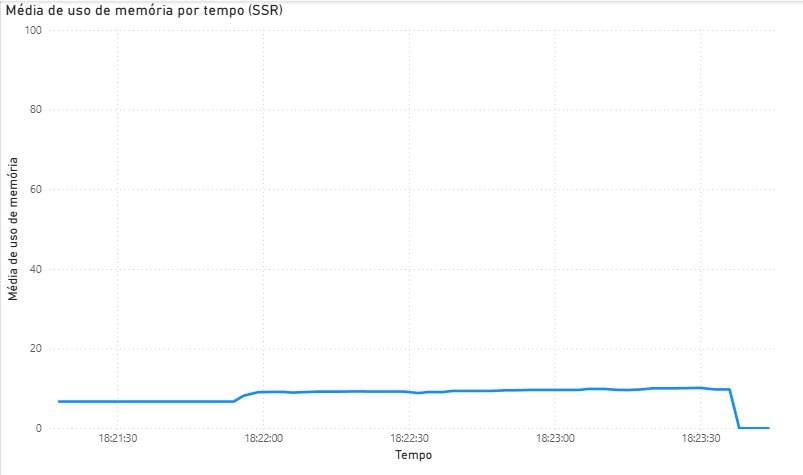
\includegraphics[width=0.9\textwidth]{media/uso_cpu_ssr.jpeg}
    \legend{Fonte: os autores.}
    \label{fig:ssr-cpu}
\end{figure}

\begin{figure}[H]
    \centering
    \caption{Média de uso de memória por tempo (\acrshort{ssr})}
    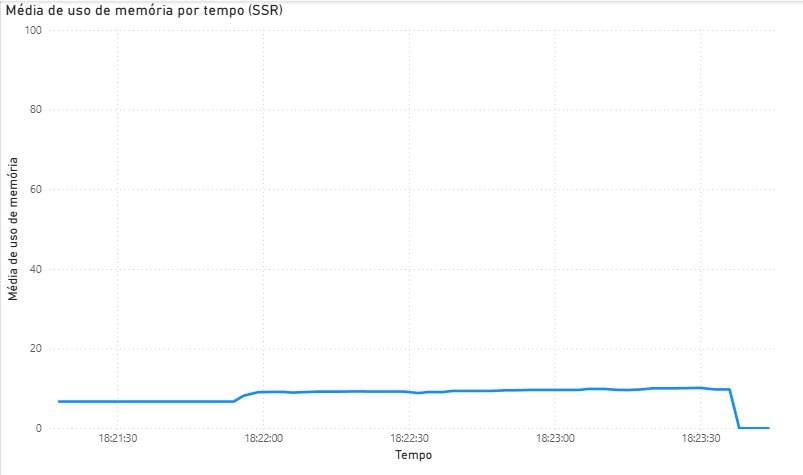
\includegraphics[width=0.9\textwidth]{media/uso_memoria_ssr.jpeg}
    \legend{Fonte: os autores.}
    \label{fig:ssr-mem}
\end{figure}

Conforme a \autoref{fig:ssr-webvitals}, as leituras de campo foram, em sua maioria, classificadas como \textit{good}. Os poucos casos de \textit{needs-improvement} concentraram-se em \acrshort{lcp} e \acrshort{inp}, e houve uma fração reduzida de \acrshort{fcp} em \textit{poor}. Esse comportamento é compatível com custos de \textit{hydration} e com elementos visuais de grande porte na dobra (imagens \emph{hero}). Em relação às metas adotadas, os resultados situam-se, em geral, próximos ou dentro dos limiares de referência: \acrshort{lcp} $\leq 2{,}5$\,s; \acrshort{cls} $\leq 0{,}10$; \acrshort{inp} $\leq 200$\,ms; \acrshort{ttfb} $\leq 800$\,ms.

\begin{figure}[H]
    \centering
    \caption{Classificação das métricas de desempenho (\acrshort{ssr}) com Web Vitals}
    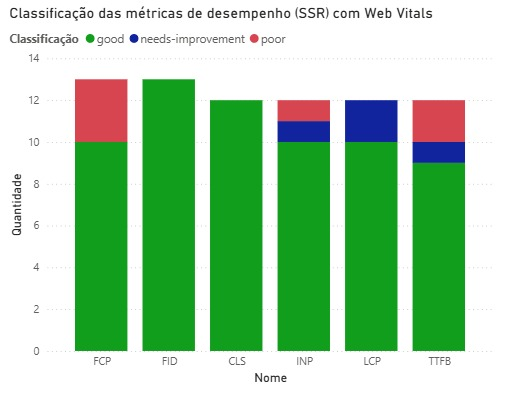
\includegraphics[width=0.9\textwidth]{media/metricas_ssr_web_vitals.jpeg}
    \legend{Fonte: os autores.}
    \label{fig:ssr-webvitals}
\end{figure}

Para explicar variações residuais e priorizar melhorias, auditamos as rotas \emph{home}, \emph{busca} e \emph{detalhe} no modo \emph{Navigation} do Chrome DevTools, considerando três indicadores: TBT, Acessibilidade e SEO. A Tabela~\ref{tab:lh-ssr} consolida as medianas observadas nos relatórios HTML anexados (\texttt{ssrMobile.html}, \texttt{ssrMobileBusca.html}, \texttt{ssrtestePage.html}).

\begin{table}[H]
\centering
\caption{Lighthouse (SSR) — mediana por rota}
\label{tab:lh-ssr}
\begin{tabular}{|l|c|c|c|}
\hline
\textbf{Rota} & \textbf{TBT (ms)} & \textbf{Acessibilidade (\%)} & \textbf{SEO (\%)} \\
\hline
Home    & 12 & 95  & 100 \\
Busca   & 10 & 99  & 100 \\
Detalhe & 0--7\footnotemark[1] & 100 & 100 \\
\hline
\end{tabular}
\end{table}
\footnotetext[1]{Variações muito baixas entre execuções; mediana $\approx$ 5\,ms.}

\noindent \textit{Leitura.}
(i) \textbf{TBT} muito abaixo da meta interna ($<200$\,ms) em todas as rotas, corroborando \acrshort{inp} em \textit{good};
(ii) \textbf{Acessibilidade} alta (95--100\%), com ajustes residuais (hierarquia de headings, foco visível, rótulos) de fácil endereçamento;
(iii) \textbf{SEO} consistente (100\%), indicando sinalização adequada (título, \emph{meta description}, \texttt{canonical}, \texttt{robots}, \texttt{viewport}) — aspecto particularmente relevante no fluxo SSR.

\subsection{Resultados Aplicação CSR}
\label{subsec:resultados-csr}

O contêiner da \emph{SPA} apresentou \textbf{CPU} muito baixa e estável, com oscilações discretas e picos inferiores a 5\% (\autoref{fig:csr-cpu}). A \textbf{memória} permaneceu praticamente constante e em patamar reduzido durante todo o ensaio, coerente com a entrega estática e a execução da lógica no cliente (\autoref{fig:csr-mem}). Não se observaram sinais de saturação.

\begin{figure}[H]
\centering
\caption{Média de uso de CPU por tempo (\acrshort{csr})}
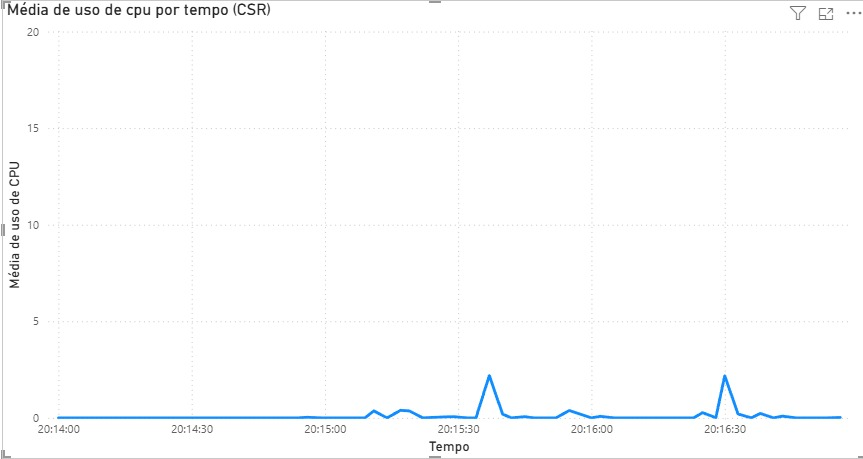
\includegraphics[width=0.9\textwidth]{media/uso_cpu_csr.jpeg}
\legend{Fonte: os autores.}
\label{fig:csr-cpu}
\end{figure}

\begin{figure}[H]
\centering
\caption{Média de uso de memória por tempo (\acrshort{csr})}
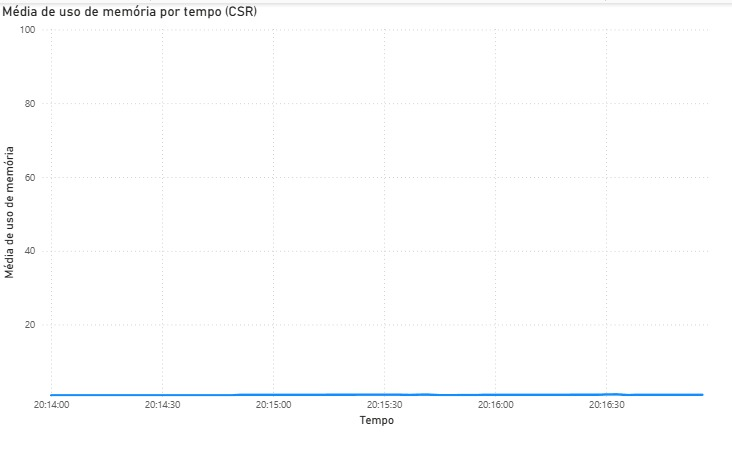
\includegraphics[width=0.9\textwidth]{media/uso_memoria_csr.jpeg}
\legend{Fonte: os autores.}
\label{fig:csr-mem}
\end{figure}

As leituras de campo indicam predomínio de \textit{good} em \acrshort{ttfb}, \acrshort{fcp}, \acrshort{lcp} e \acrshort{inp} (\autoref{fig:csr-webvitals}). O ponto fora da curva é a \acrshort{cls}, com concentrações em \textit{poor}. Esse padrão é típico de SPAs quando ocorrem \emph{layout shifts} durante a hidratação ou quando imagens/slots não reservam espaço antes do carregamento (dimensões ausentes, fontes sem \emph{preload}, inserções acima da dobra). Em relação às metas, as leituras ficaram, em geral, dentro ou próximas dos limiares de referência (\acrshort{lcp} $\leq 2{,}5$\,s; \acrshort{cls} $\leq 0{,}10$; \acrshort{inp} $\leq 200$\,ms; \acrshort{ttfb} $\leq 800$\,ms), com a ressalva da \acrshort{cls}.

\begin{figure}[H]
\centering
\caption{Classificação das métricas de desempenho (\acrshort{csr}) com Web Vitals}
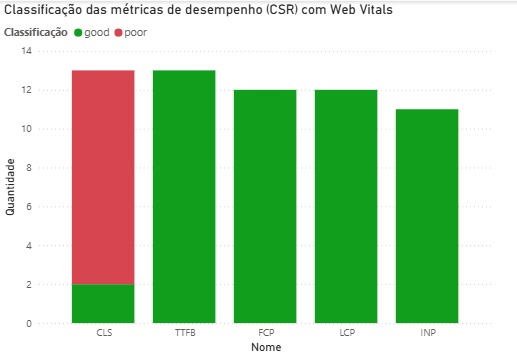
\includegraphics[width=0.9\textwidth]{media/metricas_csr_web_vitals.jpeg}
\legend{Fonte: os autores.}
\label{fig:csr-webvitals}
\end{figure}

Para explicar oscilações residuais e orientar priorizações, auditamos as rotas críticas no \emph{Chrome DevTools} (modo \emph{Navigation}), com três indicadores: TBT, Acessibilidade e SEO. Os achados indicam que o \textbf{TBT} se manteve em patamar muito baixo (dezenas de milissegundos), compatível com \acrshort{inp} em \textit{good}. Os escores de \textbf{Acessibilidade} foram altos na \emph{home} (93--94\,\%), com ajustes residuais envolvendo hierarquia de \emph{headings}, foco visível e rótulos/\textit{alt}, conforme identificado nos relatórios “Home (Web)” e “Home (Mobile)”. Já em \textbf{SEO}, a \emph{home} obteve cerca de 83\,\% (Web e Mobile), apontando oportunidades como preenchimento de \emph{meta description}, definição de \texttt{canonical}, configurações de \texttt{robots} e uso de \texttt{hreflang}, quando aplicável.

Em conjunto, os relatórios apontam que o gargalo do CSR não está em bloqueio de \emph{main thread} (TBT baixo), mas em estabilidade visual e em alguns sinais de SEO. Na prática, os seguintes ajustes tendem a capturar os ganhos: (i) reservar dimensões de imagens e \emph{cards} acima da dobra (\texttt{width}/\texttt{height} ou \texttt{aspect-ratio}); (ii) \emph{preload} de fontes e imagens \emph{hero} (com \texttt{font-display: swap}); (iii) evitar inserções DOM acima da dobra durante a hidratação; (iv) completar metadados de SEO (título/descrição/\texttt{canonical}/\texttt{robots}) e revisar indexabilidade.

Servidor praticamente ocioso (CPU e RAM baixos); \emph{Web Vitals} em boa forma para \acrshort{ttfb}/\acrshort{fcp}/\acrshort{lcp}/\acrshort{inp}, com atenção especial à \acrshort{cls}. O \emph{Lighthouse} confirmou TBT reduzido, Acessibilidade alta e SEO com melhorias de rápida implementação, coerentes com o perfil de SPA e suas responsabilidades no cliente.

\subsection{Comparação entre SSR e CSR}
\label{subsec:comparacao-ssr-csr}

Esta seção compara, de forma integrada, experiência do usuário (\emph{Web Vitals} em campo), diagnóstico laboratorial (Lighthouse: TBT, Acessibilidade e SEO) e custo operacional (CPU/Memória nos contêineres). A análise revela que a escolha arquitetônica representa um trade-off fundamental sobre onde a carga computacional deve residir: no servidor ou no cliente. A leitura está ancorada nas medianas (p50) e, quando pertinente, no p95 dos cenários home, busca e detalhe.

\begin{table}[H]
\centering
\caption{Síntese comparativa dos resultados (SSR $\times$ CSR) neste estudo}
\label{tab:comparativo-ssr-csr}
\begin{tabular}{|p{4.2cm}|p{5.2cm}|p{5.2cm}|}
\hline
\textbf{Aspecto} & \textbf{SSR (MPA/Next.js)} & \textbf{CSR (SPA/React)} \\
\hline
\textbf{CPU no servidor} & Baixa e estável (\textit{$\sim$8--13\%}), sem picos relevantes. & Muito baixa; oscilações discretas com picos $<5\%$. \\
\hline
\textbf{Memória no servidor} & Estável, variação estreita; queda apenas ao término dos testes. & Muito baixa e praticamente constante. \\
\hline
\textbf{Web Vitals (campo)} & Predominância de \textit{good}; pequenos trechos \textit{needs-improvement} em \textbf{LCP}/\textbf{INP} e fração \textit{poor} em \textbf{FCP} (páginas com imagens \emph{hero} e pós-hidratação). & \textbf{TTFB}/\textbf{FCP}/\textbf{LCP}/\textbf{INP} majoritariamente \textit{good}; \textbf{CLS} com ocorrências \textit{poor} (shifts na montagem/hidratação e elementos sem reserva de espaço). \\
\hline
\textbf{Lighthouse: TBT} & \textbf{Muito baixo} (home $\approx$12\,ms; busca $\approx$10\,ms; detalhe $\approx$5\,ms). & \textbf{Muito baixo} (ordem de dezenas de ms na home). \\
\hline
\textbf{Lighthouse: Acessibilidade} & \textbf{Alta} (95--100\%). & \textbf{Alta} (93--94\% na home). \\
\hline
\textbf{Lighthouse: SEO} & \textbf{100\%} nas rotas auditadas. & \textbf{$\sim$83\%} na home; indica metadados/sinalizações a completar. \\
\hline
\textbf{Leitura operacional} & Parte da renderização no servidor melhora \textbf{TTFB}/\emph{first paint} e favorece \textbf{SEO}; cuidado com \emph{hydration} e imagens de grande porte. & Renderização no cliente alivia o servidor e mantém \textbf{TBT/INP} baixos; requer disciplina de layout para evitar \textbf{CLS} e ajustes de \textbf{SEO}. \\
\hline
\end{tabular}
\end{table}

Entre os pontos fortes do SSR, destaca-se o tempo até a primeira resposta ou conteúdo visível. O HTML pré-renderizado acelera a exibição inicial, refletindo-se em \textit{TTFB} e \textit{FCP} consistentes e TBT residual. Essa agilidade é um fator psicológico importante, transmitindo eficiência e sendo crucial para reter a atenção do usuário nos primeiros segundos. Além disso, a descoberta e rastreabilidade são favorecidas: o SEO atingiu 100\% nas rotas auditadas, reforçando a adequação do SSR para páginas públicas e conteúdo editorial. A estabilidade visual também se mostrou sólida, com índice de \acrshort{cls} praticamente nulo, e a previsibilidade de performance é uma vantagem em redes ou dispositivos mais limitados, pois a renderização no servidor reduz o risco de tarefas longas no \emph{main thread} do navegador.

Por outro lado, o SSR apresenta alguns pontos fracos. O custo de hidratação e navegação pode afetar o desempenho, especialmente em páginas com muito JavaScript, degradando \acrshort{lcp} e \acrshort{fcp}. Além disso, a navegação subsequente, ao exigir nova requisição completa ao servidor, pode quebrar a fluidez da experiência. Embora o custo no servidor tenha sido baixo neste estudo, o modelo de processamento por requisição aumenta discretamente o uso de CPU e memória, com implicações para escalabilidade e infraestrutura. Também vale mencionar que estratégias mais avançadas, como \emph{streaming} ou \emph{Server Components}, elevam a complexidade do build e do deploy.

No CSR, os pontos fortes incluem a interatividade contínua: após o carregamento inicial, a navegação entre seções ocorre quase instantaneamente, com \acrshort{tbt} e \acrshort{inp} muito baixos, aproximando-se da experiência de um aplicativo nativo. O custo operacional também é significativamente menor, pois o servidor atua apenas como provedor de arquivos estáticos. Isso permite escalabilidade horizontal simples e integração natural com CDNs e cache.

No entanto, há desafios importantes. A estabilidade visual é comprometida — a métrica \acrshort{cls} apresentou ocorrências \textit{poor} devido a \emph{layout shifts} durante a montagem ou hidratação, especialmente quando imagens e slots não reservam espaço. Em SEO, os escores ficaram em torno de 83\%, sugerindo a necessidade de completar metadados e sinalizações essenciais. Por fim, a dependência do JavaScript no cliente torna o \acrshort{lcp} mais sensível: o tempo de carregamento inicial tende a ser mais lento, especialmente em dispositivos modestos, caso o \emph{bundle} JS não esteja bem otimizado.

Por fim, cabe uma observação sobre a ausência do FID no CSR. Nessa arquitetura, o \acrfull{fid} não é capturado de forma tradicional, pois a página precisa ser hidratada antes de se tornar interativa. Esse processo impede que o \acrshort{fid} meça corretamente a primeira interação do usuário, tornando-o menos relevante em ambientes CSR. Por esse motivo, o \acrfull{inp} é adotado como métrica alternativa, pois reflete o tempo entre a interação e a atualização visual, oferecendo uma avaliação mais precisa da interatividade em páginas dinâmicas.


\subsection{Discussão}
\label{subsec:discussao-comparativa}
Os resultados alinham-se e fornecem validação empírica para as recomendações consolidadas na literatura, confirmando que não existe uma solução universalmente superior. A escolha é uma decisão estratégica que transcende a tecnologia.

\textbf{(i) Recursos do servidor.} O \acrshort{ssr} consumiu levemente mais CPU/memória (ainda baixos), resultado do processamento por requisição. O \acrshort{csr}, por outro lado, opera como \emph{static hosting}, com custo mínimo no host, transferindo a carga computacional para o dispositivo do usuário.

\textbf{(ii) Experiência do usuário.} Em \acrshort{ssr}, a entrega inicial é perceptivelmente rápida e os escores de SEO e Acessibilidade são superiores. Em \acrshort{csr}, a interatividade após o carregamento é o grande trunfo, mas o principal cuidado é a CLS, que pode degradar a experiência.

\textbf{(iii) Coerência entre campo e laboratório.} Os \textit{Web Vitals} em campo e o TBT do Lighthouse convergiram, indicando baixo bloqueio de \emph{main thread} em ambos os modelos. As divergências em CLS (CSR) e SEO(CSR $<$ SSR) são áreas classicamente sensíveis à estratégia de renderização.

\subsection{Implicações práticas}
A decisão entre as arquiteturas deve ser ponderada à luz dos objetivos do produto, das expectativas do usuário e das capacidades da equipe de desenvolvimento.
\begin{itemize}
    \item \textbf{Priorizar SSR} para aplicações de conteúdo, como portais de notícias, plataformas de e-commerce e blogs, onde a otimização para mecanismos de busca (SEO) é vital, e a velocidade da primeira impressão (TTFB e FCP) é um fator determinante para o sucesso do negócio.
    \item \textbf{Priorizar CSR} para aplicações web ricas e complexas, como dashboards analíticos, sistemas de gestão interna (ERPs) e plataformas de software como serviço (SaaS), que geralmente são acessadas após autenticação e onde a fluidez da interatividade contínua (INP) é mais valorizada do que a indexabilidade de páginas individuais.
\end{itemize}

\subsection{Ajustes recomendados}

\acrfull{ssr} (mitigar \acrshort{lcp}/\acrshort{inp}). Otimizar e dimensionar imagens (usar \texttt{priority} para \emph{hero} e \emph{lazy} abaixo da dobra), considerar \emph{streaming}/\emph{partial hydration}/\emph{Server Components}, reduzir \acrshort{js} não crítico e declarar \texttt{preload}/\texttt{dns-prefetch} para recursos essenciais. \\

\acrfull{csr} (mitigar \acrshort{cls} e elevar \acrshort{seo}). Reservar dimensões de mídia (\texttt{width}/\texttt{height} ou \texttt{aspect-ratio}); evitar inserções acima da dobra durante a hidratação; \texttt{font-display: swap} com \emph{preload} de fontes e imagens \emph{hero}; placeholders do tamanho final; completar metadados e sinalizações (\emph{title}/\emph{description}/\texttt{canonical}/\texttt{robots}/\texttt{hreflang}, quando aplicável).

\subsection{Síntese}
No cenário testado, \acrshort{ssr} e \acrshort{csr} entregaram boa experiência de uso com baixa pressão de recursos. A \acrfull{ssr} destacou-se por \acrshort{seo} e exibição inicial mais previsível, sendo ideal para aplicações de conteúdo. A \acrfull{csr} reduziu o custo no servidor e garantiu interatividade fluida, com a contrapartida de maior propensão a \acrshort{cls} e desafios de \acrshort{seo}, mostrando-se adequada para aplicações ricas e logadas. A decisão final deve considerar o perfil de tráfego, a exigência de descoberta e o tipo de interação, aplicando as otimizações para mitigar os pontos fracos identificados em cada abordagem.
